\chapter{Physics}
A custom physics engine was created for the game. The \textbf{physics.js} file contains the physics needs for the game.

First of all, physics objects are created. Two were defined for this game:
\begin{itemize}
	\item \textit{RectObject}, which has a width and height
	\item \textit{CircObject}, which hs a radius
\end{itemize}
Both of these 2 objects have a position (array of size 2, representing the x and y coordinates on the screen) and a velocity (array of size 2, representing the x and y velocity).

Some function which were defined and used were the following:
\begin{itemize}
	\item \textit{euclidean\un distance}: Given 2 points, it gets the euclidean distance between them
	\item \textit{CollisionRectCirc}: Takes a rectangle and a circle and returns if they intersect or not. Note: This does not consider the possibility of the circle being completely inside the square or vice versa. This function returns a collision type, whether the circle intersects with the top, bottom, left, bottom left, top right, etc, of the rectangle. Use fro collision between balls or bullets or powerups with the walls, bricks platform or other balls, as appropriate (for example: platform with brick collision does not make sense to check for).
	\item \textit{CollisionCircCirc}: Given 2 circles, checks if the 2 circles intersect by computing the distance between them and checks that this is smaller than te sum of their 2 radii.
	\item \textit{getDirectionVector}: Given 2 points, this returns a normalised direction vector from one position to the other. Used for when 2 balls collide with each other.
	\item \textit{multiply}: Multiplies a 2D vector by a scalar
	\item \textit{changeVelocityFromPoint}: While retaining the magnitude of the velocity vector given, it redirects such that it is now moving away from a specific point. This is used for when the ball collides with th platform. A point under the platform is used to shoot the ball away from the platform. Visually:
	\begin{figure}[H]
		\centering
		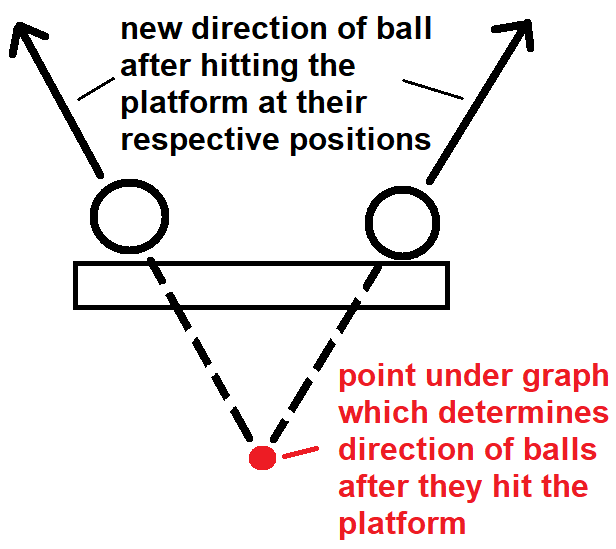
\includegraphics[width=0.3\textwidth]{Images/BallPlatform.png}
		\caption{Explanation of how ball rebounds off of platform}
	\end{figure}
	\item \textit{move}: Increments position of an object by its velocity
	\item \textit{moveMultiply}: Increments position of an object by its velocity vector multiplied by some amount
\end{itemize}

The physics engine is used within the animate function in \textbf{script.js}. The physics objects are initialised at the start for each object needed. Then within the animate function, the platform first moves, by checking user input of the right and let arrows. Then the ball and any other item which has a velocity is moved using the \textit{move} function. Afterwards, the collisions are computed and actions are taken accordingly. If a brick is hit, this is removed from the scene graph and the ball's velocity is rebounded accordingly. If a wall is hit the ball also rebounds. Then the actual nodes in the scene graph are moved according to the position of their respective physics objects.

When the game starts the ball is positioned in the middle of the platform, which can move left to right with the ball. Pressing spacebar releases the ball. Holding spacebar increases the launch velocity of the ball. If the ball falls down the pit, then it is reset on top of the spacebar. At 3 deaths, or when the player destroys all the bricks, the game is reset.